\documentclass[12pt]{article}
\usepackage{graphicx}
\usepackage{hyperref}
\usepackage{fancyhdr}
\usepackage{setspace}
\pagestyle{fancy}
\fancyhead{}
\fancyfoot{}
\fancyfoot[C]{-\thepage-}
\fancyfoot[L]{ID:997900158}
\fancyfoot[RO]{MPM406 - Random Clinical Trial}
\renewcommand{\footrulewidth}{0.4 pt}
\renewcommand{\headrulewidth}{0 pt}

\hypersetup{colorlinks = true, linkcolor = blue, citecolor = blue}
\title{Investigation into the effect of growing food onsite on the incidence of cryptosporidiosis in California Ranching households}
\author{Student ID: 997900158}
\date{\today}
\begin{document}
	\maketitle
	\begin{abstract}
		This cohort study's objective was to investigate the relationship between California ranchers growing food onsite and incidence of cryptosporidiosis in their household.
		Ranchers from a CDFA database were sent an initial questionnaire, followed up by a visit from a nurse practitioner to collect information on various household, occupational, and dietary variables.


		Households that grew more than 50\% their food  on site were 3.01 (95\% CI: 2.81 - 3.21)times more likely to experience a cryptosporidiosis event each year than those who did not grow more than 50\% of food onsite.

	\end{abstract}

\onehalfspace
	\section{Introduction} 
		Kaiser Permanente is a managed care consortium based in northern California. It has almost 15,000 physicians operating in 650 facilities, and servesnearly 9 million members \cite{Rauber}.


	\section{Methods} 
		post menopausal women (defined as no menstural cycle for 12 months) will be enrolled by their primary care physician at Kaiser Permanente facilities spread over 9 states.

		Patients were randomised using a centralised allocation procedure, with both patient and physician blinded to allocation method. 
		On identifying a possible study subject, a full physical examination and medical history was taken, and where possible validated with a central database of historical medical records maintained by Kaiser Permanente.

	\subsection{Statistical Evaluation}
		Cox proportional hazard models were used with time to event as response and various covariates discussed above as predictors, with a household level random effect included.
		The baseline hazard was modified to follow a weibull distribution to reflect the time dependence of risk for cryptosporidiosis, with an increased risk occurring with the presence of young calves following calving start date. 
		Incidence density rates were calculated for all strata of the covariates with findings indicated in \hyperref[table2]{Table 2}.



	\section{Results}


	\section{Discussion} 


	\subsection{Strengths and Limitations}
		Data quality was a strenth of this study.
		Cross validating the patients oral medical histories with the actual recorded histories from the Kaiser Permanente central databases ensures accuracy and reduces recall bias.
		
	\section{Figures}

\begin{figure*}[h!]
	\centering
	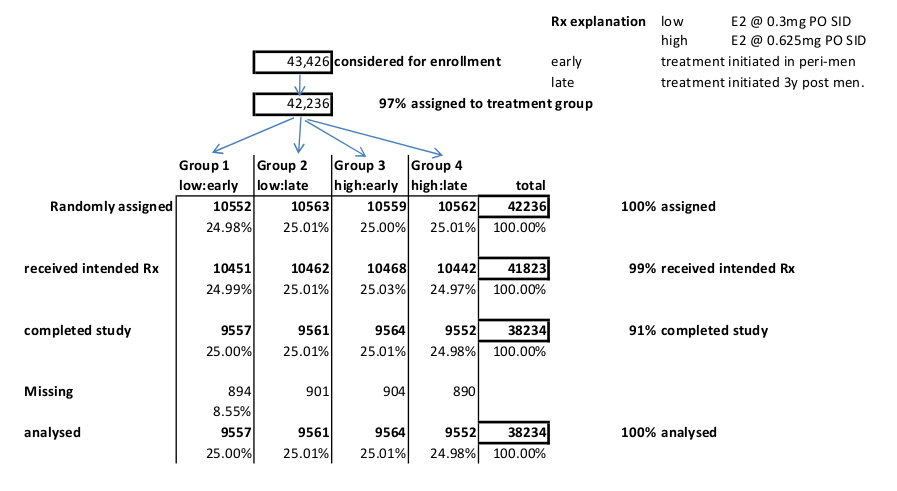
\includegraphics[scale=0.3]{figure1.jpg}
	\caption{Flow Diagram showing proposed Biological Rationale for study, including exposure, outcome and covariates }
	\label{figure1}
\end{figure*}

\begin{figure*}[h!]
	\centering
	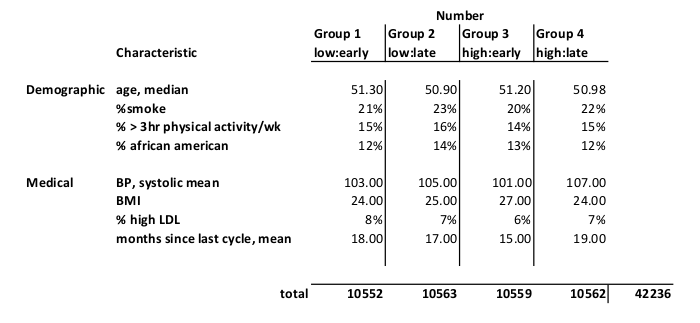
\includegraphics[scale=0.5]{table1.jpg}
	\caption{Characteristics of study participants and sample size calculations.}
	\label{table1}
\end{figure*}
 
\begin{figure*}[h!]
	\centering
	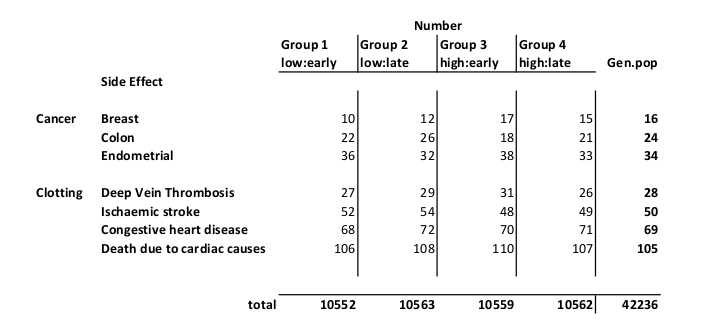
\includegraphics[scale=0.5]{table2.jpg}
	\caption{Risk Ratios (RR) for the association between growing food onsite and cryptosporidiosis.}
	\label{table2}
\end{figure*}

\begin{figure*}[h!]
	\centering
	\includegraphics[scale=0.6]{sample.jpg}
	\caption{Sample size function and calculation output from R. Calculations agrees with Epi Info when continuity correction was applied.}
	\label{sample}
\end{figure*}

\clearpage
\bibliographystyle{unsrt}
\bibliography{women}



\end{document}

%%%%%

% interactoins - 
%% make streamlined as possible. but need at least one confounder, not necc any interactions, can say did not find any (kim paper for technique - none stat sig so not included). potential effect modify - wualitative. 
% if include need to show OR with and without interactions.
% table 1 - cats in study,. throw in other factors that wont include - make them the same. e.g. age w exposure outcome and not on causal path. - no sig p value. 
% fig 1 - exposure b \emph{Bartonella sp.} , outcome ev.

% diagram bartonella causing uveitis, age associated w bartonella and uveitis (double ended arrow.) then show in table.( anythign in table that same do not need to have in diagram.
